\documentclass[border=10pt]{standalone}
\usepackage{tikz}
\usetikzlibrary{matrix, positioning}

\begin{document}
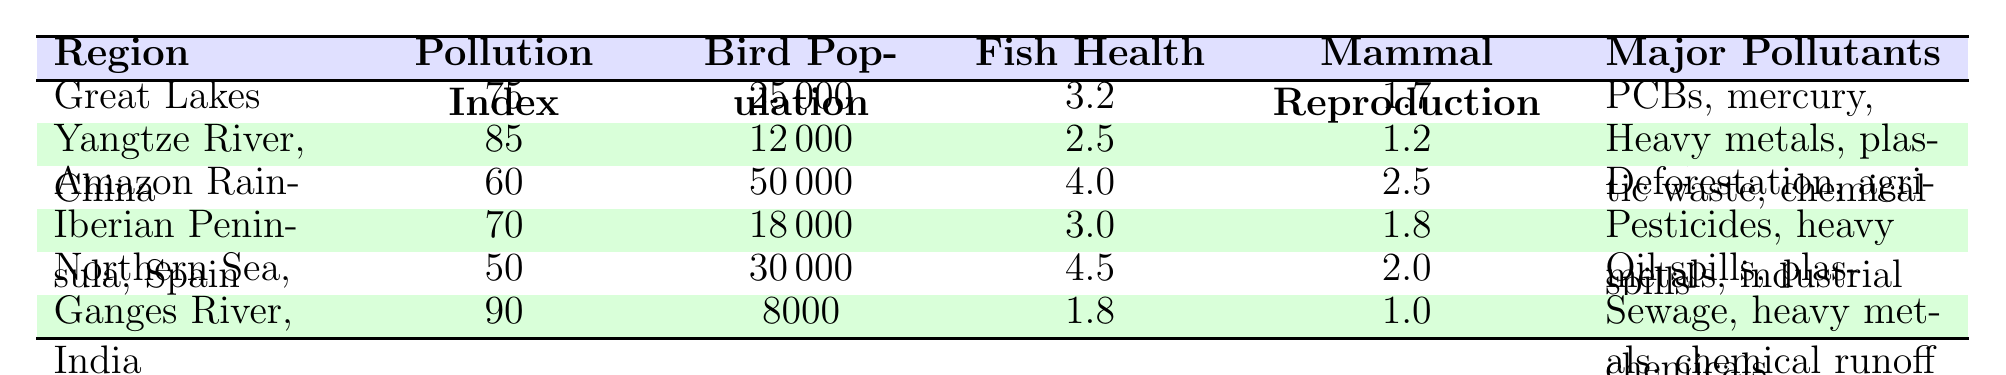
\begin{tikzpicture}
    \matrix (m) [
        matrix of nodes,
        row sep=0pt,
        column sep=0pt,
        nodes={draw=none, anchor=center, inner xsep=6pt, inner ysep=4pt, font=\Large, text depth=.25ex, text height=1.5ex},
        column 1/.style={nodes={text width=3.7cm, align=left}},
        column 2/.style={nodes={text width=3.2cm, align=center}},
        column 3/.style={nodes={text width=3.5cm, align=center}},
        column 4/.style={nodes={text width=3.0cm, align=center}},
        column 5/.style={nodes={text width=4.2cm, align=center}},
        column 6/.style={nodes={text width=4.4cm, align=left}},
        row 1/.style={nodes={fill=blue!12, font=\Large\bfseries}},
        row 3/.style={nodes={fill=green!15}},
        row 5/.style={nodes={fill=green!15}},
        row 7/.style={nodes={fill=green!15}}
    ] {
        Region & Pollution Index & Bird Population & Fish Health & Mammal Reproduction & Major Pollutants \\
        Great Lakes Basin, USA & 75 & 25\,000 & 3.2 & 1.7 & PCBs, mercury, heavy metals \\
        Yangtze River, China & 85 & 12\,000 & 2.5 & 1.2 & Heavy metals, plastic waste, chemical runoff \\
        Amazon Rainforest, Brazil & 60 & 50\,000 & 4.0 & 2.5 & Deforestation, agricultural runoff, oil spills \\
        Iberian Peninsula, Spain & 70 & 18\,000 & 3.0 & 1.8 & Pesticides, heavy metals, industrial waste \\
        Northern Sea, Norway & 50 & 30\,000 & 4.5 & 2.0 & Oil spills, plastic debris, marine chemicals \\
        Ganges River, India & 90 & 8000 & 1.8 & 1.0 & Sewage, heavy metals, chemical runoff \\
    };
    
    \draw[line width=1pt, black] (m-1-1.north west) -- (m-1-6.north east);
    \draw[line width=1pt, black] (m-1-1.south west) -- (m-1-6.south east);
    \draw[line width=1pt, black] (m-7-1.south west) -- (m-7-6.south east);
\end{tikzpicture}
\end{document}
